%&platex --translate-file=cp1250pl
\documentclass[times]{jtitauth}
\graphicspath{{Figures/}}  % Location of the graphics files (set up for graphics to be in PDF format)

\begin{document}

\title{Data Driven Automated Algorithmic Trading}

\author{Gabriel Gauci Maistre}

\markboth{Gabriel Gauci Maistre}
{Data Driven Automated Algorithmic Trading}

\maketitle

\begin{abstract}
Various existing stock market price forecasting methods were analysed in this report. Three methods were applied towards the problem making use of Technical Analysis, these were Time Series Analysis, Machine Learning, and Bayesian Statistics. Through the results of this report, it was found that the Efficient Market Hypothesis remains true, that past data does not contain enough useful information to forecast future prices and gain an advantage over the market. However, the results proved that Technical Analysis and Machine Learning could still be used to guide an investors decision. It was also found that the Random Walk Hypothesis was not necessarily true, as some stocks showed signs of auto and partial correlation. A common application of technical analysis was demonstrated and shown to produce limited useful information in beating the market. Based on the findings, a number of automated trading algorithms were developed using machine learning and backtested to determine their effectiveness.
\end {abstract}

\begin{keywords}
machine learning, time series analysis,
probabilistic, bayesian, statistics,
inference, algorithmic trading\
\end{keywords}

\section{Introduction}

The stock market retains its status as a prime location for investors to invest in the market and earn a profit, however this is not always easy due to the constantly thriving and changing nature which follows the stock market. Investors are constantly presented with numerous profit potential opportunities, however without intensive planning and analysis, these opportunities could easily turn into losses. This means that it is crucial for every investor to carry out stock market ananlysis prior to any investment by monitoring past price movements in order to forecast future trends. Even though past data is not a clear indication of future movement, it is still proven to provide some useful insite.

In this paper, we investigate the Efficient Market Hypotheses (EMH), and the Random Walk Hypothesis (RWH) in the context of stock market forecasting and trading. For the purpose of benchmarking the performance of the algorithms, a total of five stocks were randomly selected from a basket of uncorrelated stocks were selected. These were MSFT, CDE, NAVB, HRG, and HL. Our key findings are as follows:

\begin{enumerate}
  \item We found strong auto and partial correlation in the stocks studied, disproving the RWH.
  \item We found the EMH to be true, as although the automated trading algorithm made a large profit, it was not sufficient to beat the returns of the market.
  \item Time series analysis was found to be a weak factor in forecasting financial stocks.
  \item Bayesian statistics was a strong contender as a forecasting method.
  \item Machine learning was found to be the best method of forecasting using both classification and regression methods. 
  \item We found regression methods of machine learning to fair better than classification methods when implemented and backtested.
\end{enumerate}

\section{Experiments}
A data set containing end of day stock prices, dividends, and splits for 3,000 US companies, curated by the Quandl community[1], and released into the public domain, was used. The date column in the CSV file was loaded into memory, and said column was converted to a date data type. The data frame was then sorted using the date column, starting from the oldest date, ending with the latest. The date column was also set to the index. The data frame was split into two, the training data set consisting of 80\%, and the test data set consisting of 20\% of the original data frame.

\subsection{Time Series Analysis}
The selected stocks was extracted from the data set and stored in a data frame. The log returns of the stocks were calculated by calculating the logarithm of the stock's adjusted close price divided by the following day's adjusted close price. The resulting values from the calculation were then stored in a new column in the data frame and all infinite values were dropped from the series.

The random walk theory suggests that stock price changes have the same distribution and are independent of each other, so the past movement or trend of a stock price or market cannot be used to predict its future movement. In short, this is the idea that stocks take a random and unpredictable path. As can be seen in figure 1, the correlation plots show this theory to be false and that past movement is related to future movement.

\begin{figure}[!hbp]
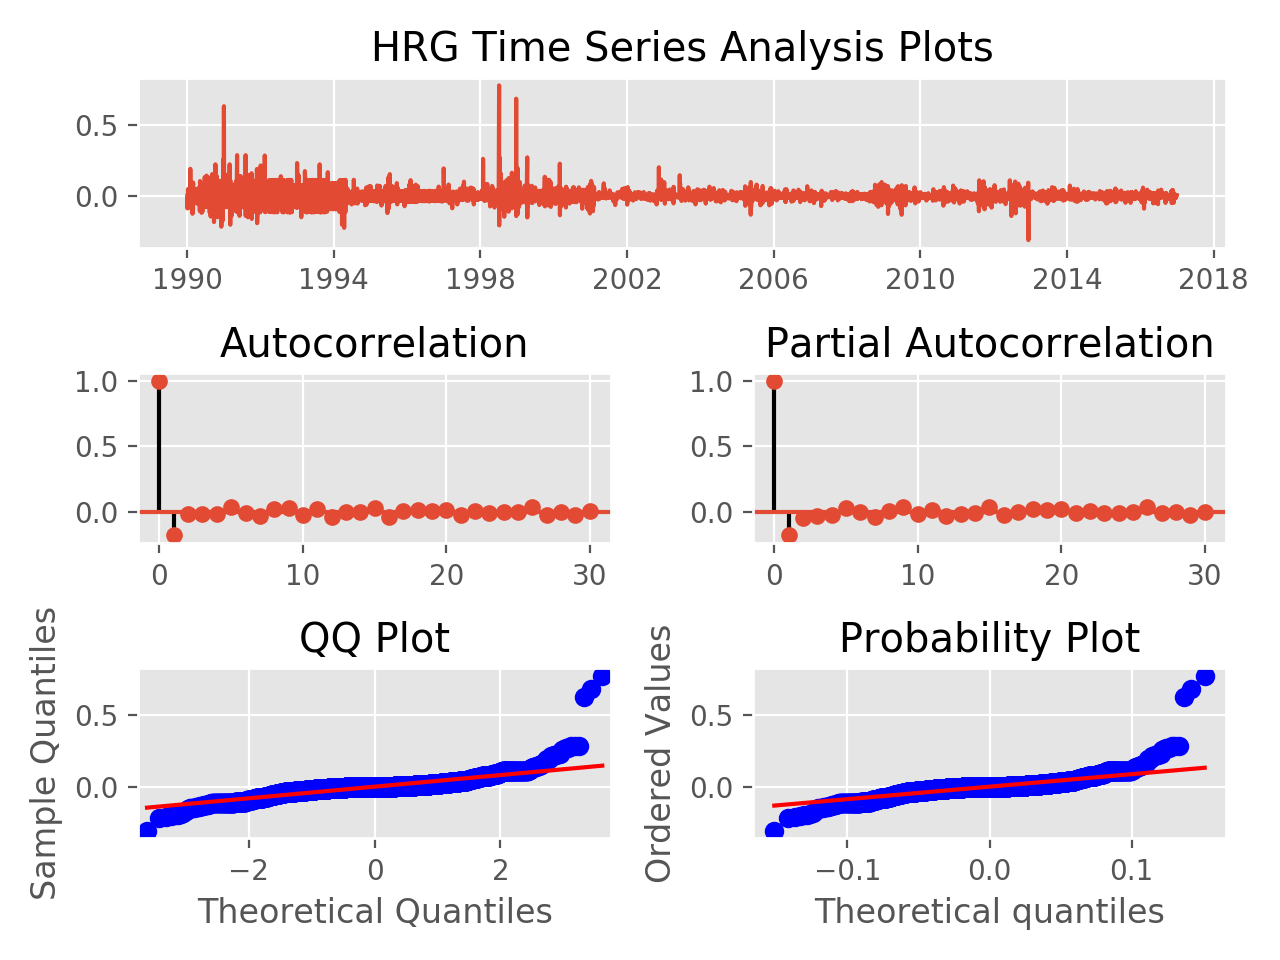
\includegraphics[width=0.5\textwidth]{HRG-time-series.png}
\caption{HRG Time Series Analysis}
\end{figure}

ARMA faired the best than the rest of the algorithms in predicting stock price returns, having the lowest difference in sharpe ratios based on the original price returns and in-sample predicted price returns, however still failed to achieve a good fit in the in-sample tests. The series was fitted to an ARMA(p, q, r) model with an order selected based on the lowest AIC. No constants were passed to the ARMA model. The exact loglikelihood for the fit of the ARMA model was maximized via the Kalman Filter. As can be seen in the time series analysis plots, ARMA showed to have very heavy tails in the QQ and probability plots. The algorithm predicted an abnormal sharp decline at the start of the forecast and showed diminishing returns over time, as was evident in figure 2.

\begin{figure}[!hbp]
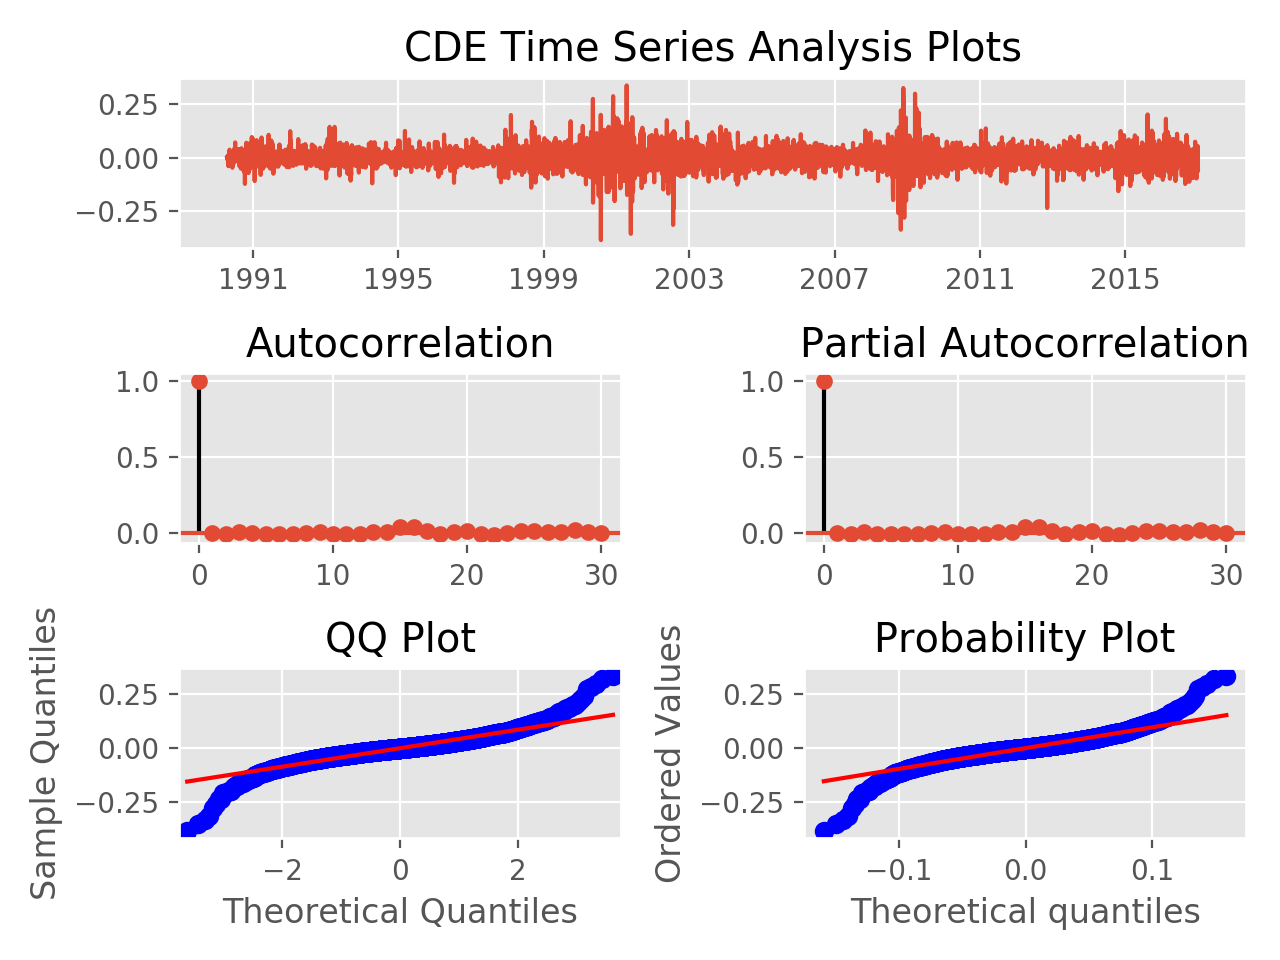
\includegraphics[width=0.5\textwidth]{CDE-ARMA-time-series.png}
\caption{CDE ARMA Time Series Analysis}
\end{figure}

\subsection{Machine Learning}

The random forest was fit with bootstrap samples when building the trees, while all the weights associated were set to 1. The 'gini' function to measure the quality of a split, and no maximum depth of the tree was set, allowing the nodes to expand until all leaves are pure or until all leaves contain less than the minimum split samples. The number of features to consider when looking for the best split was the square root of the number of passed, and no limit on the maximum leaf nodes for growing trees was set. A threshold of 1e-7 was used to terminate the tree growth to determine if a node is a leaf, if the impurity of a node is below the threshold, the node is a leaf. The minimum number of samples required to be at a leaf node was set to 1, and the minimum number of samples required to split an internal node was set to 2. The minimum weighted fraction of the sum total of weights (of all the input samples) required to be at a leaf node was set to 0, and the number of trees in the forest was set to 10. The number of jobs to use for the computation was set to 1, making use of only 1 CPU core, and out-of-bag samples to estimate the generalization accuracy were not used. The verbosity of the tree building process was not controlled, and the random number generator used by the model was that of Numpy's RandomState. The model was built using a cold start by not making use of the previous call to fit and add more estimators to the ensemble, meaning a whole new forest was fit instead. 

\begin{table}
    \centering
        \begin{tabular}{ | l | l | l | | l | l | l | p{5cm} |}
        \hline
        Ticker & Precision & True - & False - & True + & False + \\ \hline
        MSFT & 0.77 & 493 & 131 & 547 & 190 \\ \hline
        CDE & 0.79 & 566 & 145 & 503 & 132 \\ \hline
        NAVB & 0.76 & 590 & 164 & 332 & 128 \\ \hline
        HRG & 0.75 & 554 & 210 & 462 & 134 \\ \hline
        HL & 0.81 & 581 & 101 & 509 & 169 \\
        \hline
        \end{tabular}
    \caption{Random Forest Classification Results}
\end{table}

\subsection{Bayesian Statistics}

The last 500 rows of the selected stocks were extracted from the data set and stored into a data frame. The log returns were calculated by dividing each day’s adjusted close with the adjusted close of the following day, in logarithmic form. The resulting values from the said calculation were then stored in a new column in the data frame and all infinite values were dropped from the series. The sharpe ratio of the original and predicted price returns was calculated to serve as an accuracy score in the in-sample tests. The model returns were modeled with a Student-t distribution with an unknown degrees of freedom paramater, and a scale paramater determined by a latent process. The algorithm achieved a good fit in the in-sample tests, having very similar sharpe ratios based on the original price returns and in-sample predicted price returns.

\begin{figure}[!hbp]
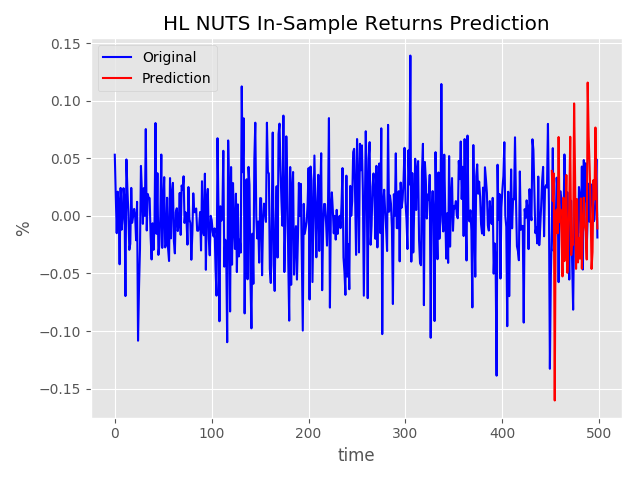
\includegraphics[width=0.5\textwidth]{HL-NUTS-In-Sample-Returns-Prediction.png}
\caption{HL NUTS In-Sample Returns Prediction}
\end{figure}

\subsection{Strategy}

We evaluated both classification and regression methods for algorithmic trading, in which it was evident that regression methods were superior to those of classification. An ordered dictionary was used to store the day's close price for each stock as the backtester simulated each trading day. The algorithm was only allowed to run once there was enough price data, the amount chosen was 50. The 15 and 50 day SMAs were calculated and each stored in an array. The two arrays were converted into an array of tuples, where the i-th tuple contains the i-th element from each of the argument sequences or iterables. The independent variables, the SMAs, and the dependant variables, the close prices for the particular stock, were passed to the machine learning algorithm to predict the next day's close price. An order was placed on a stock if the predicted price was higher the current day's price. A stop loss of 80\% was placed on each position. 

When tasked with predicting rises in stock prices, the algorithm did fairly well, marking a slightly lower total return of 43\%. The agorithm also underperformed immensely when tasked at also predicting stock price falls, marking a negative total return of -80.4\%. To compensate for this, a stop loss was added to sell all positions if the stock in question falls below -20\%, this resulted in a profit of 83.7\%.

\begin{table}[!hbp]
    \centering
        \begin{tabular}{ | l | l | l | | l | l | l | p{5cm} |}
        \hline
        Starting Capital & \$100,000 \\ \hline
        Total Capital Used & \$229,547.84 \\ \hline
        Sharpe Ratio & 0.420 \\ \hline
        Portfolio Value & \$183,714.616 \\ \hline
        Algorithm Period Return & 0.837 \\ \hline
        Benchmark Period Return & 1.008 \\ \hline
        Algorithm Volatility & 0.373 \\ \hline
        Benchmark Volatility & 0.156 \\
        \hline
        \end{tabular}
    \caption{Machine Learning Regression Strategy With Stop Loss}
\end{table}

\begin{figure}[!hbp]
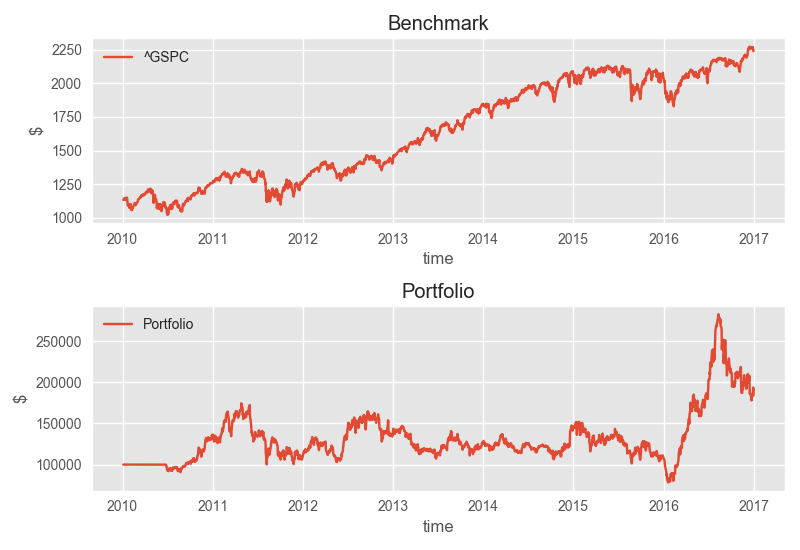
\includegraphics[width=0.5\textwidth]{MLR-Portfolio-Benchmark-Stop-Loss.png}
\caption{Machine Learning Regression Strategy With Stop Loss}
\end{figure}

\section{Related work}

There is a growing demand for forecasting interest rates, as financial researchers, economists, and players in the fixed income markets seek to find the best method to get ahead of the market. A financial model was developed to forecast short-term interest rates, implicit yield on 91 day treasury bill, overnight MIBOR rate, and call money rate.[2] Radha et al. made use of univariate models to forecast the short-term interest rates. These models include Random Walk, ARIMA, ARMA-GARCH, and ARMA-EGARCH. They selected the best peforming model by considering a six year period starting from 1999. Radha et al. showed evidence that GARCH models are best suited for forecastint when applied towards time series having volatility clustering effects. It was their firm belief that ARIMA-EGARCH is the most appropriate forecasting model for these circumstances.

Darrat et al. set out to investigate with the use of new daily data, whether prices in the two Chinese stock exchanges (Shanghai and Shenzhen) follow a random walk process as required by market efficiency.[3] Two different approaches were applied, the standard variance-ratio test, and a model-comparison test that compares the ex post forecasts from a naive model with those obtained from several alternative models such as ARIMA, GARCH, and ANNs. To evaluate ex post forecasts, Darrat et al. made use of several procedures including root-mean-square error (RMSE), mean absolute error (MAE), uncertainty coefficient, and encompassing tests. It was concluded that the model-comparison approach yielded results which were quite strongly rejected the RWH in both Chinese stock markets when compared with the variance-ratio test. Darret et al. recommended the use of ANNs, as their results showed strong support for the model as a potentially useful factor for forecasting stock prices in emerging markets.

A vast majority of academics tend to predict the price of stocks in financial markets, however most models used are flawed and only focus on the accurate forecasting of the levels of the underlying stock index. There is a lack of studies examining the predictability of the direction of stock index movement. Given the notion that a prediction with little forecast error does not necessarily translate into capital gain, the authors of this research attempt to predict the direction of the S\&P CNX NIFTY Market Index of the National Stock Exchange, one of the fastest growing financial exchanges in developing Asian countries.[4] Machine learning models such as random forest and SVMs, differ widely from other models, and are making strides in predicting the financial markets. Kumar et al. tested classification models to predict the direction of the markets, by applying models such as linear discriminant analysis, logistic regression, ANNs, random forest, and SVM. Their evidence shows that SVMs outperform the other classification methods in terms of predicting the direction of the stock market movement, and that the random forest model outperforms other models such as ANNs, discriminant analysis, and logistic regression.

Creamer et al. developed an automated trading algorithm making use of multiple stocks relying on a layered structure consisting of a machine learning algorithm, an online learning utility, and a risk management overlay.[5] The machine learning algorithm which they made use of was an Alternating Decision Tree (ADT) implemented with Logitboost. Their algorithm was able to select the best combination of rules derived from well known technical analysis indicators, and the best peramaters of the indicators in question. Additionally, their online learning layer was also able to combine the output of several ADTs, suggesting a short or long position. Finally, the risk management layer in which they implemented, was able to validate the trading signal once it exceeds a specified non-zero threshold and limit the application of their trading strategy when it is not profitable. They tested the expert weighting algorithm with data of 100 randomly selected companies of the S\&P 500 index during the period 2003–2005. They found that their algorithm generated abnormal returns during the test period. Their experiments show that the boosting approach was able to improve the predictive capacity when indicators were combined and aggregated as a single predictor. Furthermode, their results indicated that the combination of indicators of different stocks were adequate in order to reduce the use of computational resources, while still maintaining an adequate predictive capacity.

In their paper, Hoffman et al. introduced the NUTS model, an improvement to the HMC model. The NUTS model is a model of MCMC family of algorithms, in which its main focus is to avoid the random walk behavioir and sensitivity to correlated paramaters affecting many other MCMC models. Hoffman et al. achieved this by taking a series of steps informed by first-order gradient information.[6] In their study, they claim HMC to be flawed as its performance is highly sensitive to two user-specified parameters, the step size, and the desired number of steps. NUTS is an improvement from HMC as it eliminates the need for the researcher to set the number of steps, and works by building a set of likely candidate points which span a wide swath of the target distribution, stopping automatically when it starts to double back and retrace its steps. They achieved all of this by making use of a recursive algorithm.

\section{Conclusion}
Three financial forecasting methods were presented in this report, two of which showed little to no potential of ever producing any statistically significant result when the correct methodology was applied. The third method, machine learning, showed some potential in the tests carried out, which is why this method was built into an automated algorithmic strategy to trade with. The algorithm proved to be successful in forecasting future prices, using both classification and regression methods. However, the backtesting proved this method to fail in forecasting price falls. Once this factor was removed from the equation, the algorithms were very successful and reported a profit by the end of the test. This is however not always ideal as stocks which could fall in price could be catastrophic to the strategy. A stop loss would be ideal in insuring that no positions are held in downward falling stocks. It was also evident that regression methods were more successful in forecasting future price movements when compared to classification methods.

If there is anything that this report shows, is that profitable stock market prediction is an extremely tough problem. Even though the strategies reported a profit by the end of the backtest, they still did not beat the market. Whether it is at all possible to use such methods to outperform the market’s returns, ultimately remains an open question. These findings support the Efficient Market Hypothesis, proving that casual investors are better off investing in passive buy and hold strategies consisting of index funds and ETFs. However, there was some evidence found showing that the Random Walk Hypothesis does not hold true for all cases, as some stocks did show signs of repeating trends.

\section*{Acknowledgements}

The author would like to express his special thanks of gratitude to my supervisor, Alan Gatt, for the patient guidance, encouragement, and advice he has provided throughout my time as his student. He would also like to thank Luke Vella Critien, for guiding him towards the right parth in the early stages of my research and for recommending Alan Gatt as my tutor. The author's gratitude is also extended to Emma Galea and Miguel Attard for their valuable input while carrying out his research. Completing this work would have been all the more difficult were it not for the support and friendship provided by the other members of the Malta College of Arts, Sciences, and Technology, and the institute of Information and Technology. The author is indebted to them for their help. Finally, the author wishes to express his very profound gratitude to his family for providing him with unfailing support and continuous encouragement throughout his years of study and through the process of researching and writing this thesis. This accomplishment would not have been possible without them. 

\begin{thebibliography}{99}

\bibitem{1}Quandl. Wiki eod stock prices, 2017.
\bibitem{2}S. Radha and M. Thenmozhi. Forecasting short term interest rates using arma, arma-garch and arma-egarch models. {\it Indian Institute of Capital Markets 9th Capital Markets Conference Paper}, January 2006.
\bibitem{3}Ali F. Darrat and Maosen Zhong. On testing the random walk hypothesis: A model-comparison approach, 2001.
\bibitem{4}Manish Kumar and M. Thenmozhi. Forecasting stock index movement: A comparison of support vector machines and random forest, June 2016.
\bibitem{5}Germ ́an G. Creamer and Yoav Freund. Automated trading with boosting and expert weighting. {\it Quantitative Finance}, Vol. 4(No. 10):pp. 401–420, April 2010.
\bibitem{6}Matthew D. Hoffman and Andrew Gelman. The no-u-turn sampler: Adaptively setting path lengths in hamiltonian monte carlo. {\it Journal of Machine Learning Research}, 15, 2014.
\end{thebibliography}

\end{document}
